\scanpage{27}
$c$ \inserted{\unsure{très régulière}} sur $P$ il existe un isom et un seul $u$ \deleted{tel que $u(\widehat c)$} prolongeant $u_3$ et tel que $u(\widehat c)=C$.
\figure{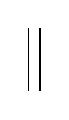
\begin{tikzpicture}\draw (0,0)--(0,-.8);\draw (.15,0)--(.15,-.8);\end{tikzpicture}}
Donc corr. biunivoque entre

a) les solutions du Pb initial, à isom près (NB la cat. des solutions est \uline{rigide})

b) $(P,\sigma)$ étant choisi can. comme expliqué, avec $u_2$, l'ens des \inserted{isom} $u_3$ qui \unsure{prolongent} $u_2$ -- qui forment donc un \inserted{pseudo} torseur sous
\[
\Gamma(X,\Omega^{\otimes2})
\]
c) L'ens des connexions $c$ sur $P$ \deleted{qui} telles que \inserted{$\widehat c$ soit dans} \deleted{soit dans une} une orbite donnée de $G_2$ opérant sur $\operatorname{Conn}^*(P)$, \deleted{\unsure{et qui soit}}

\diagram{\begin{tikzcd}
\operatorname{Iso}^{!}_{\infty} \arrow[d] \arrow[dr] & \\
\operatorname{Sol} \arrow[r,"\sim"] \arrow[dr,"\sim"] & \operatorname{Iso}^{!}_{3} \\
\unsure{\mathrm{rig}} & \operatorname{Conn}^{*}P\;!
\end{tikzcd}}
\[
\deleted{\unsure{u(C)=\widehat c}}\qquad g\widehat c=
\]
\diagram{\begin{tikzcd}
\Omega \arrow[r] & \widehat S\otimes\Omega^1_{X/S}
\end{tikzcd}}
\[
\prod_{i\geq0}\Omega^{\otimes i}\otimes\Omega^1_{X/S}
\]
\[
\Omega^{-1}+\mathcal O+\Omega
\]
\figure{\begin{tikzpicture}[x=.55cm,y=.55cm]
\draw (0,0)--(4.9,3.5)--(6.7,3.8)--(6.9,5)--(10,5.4);
\end{tikzpicture}}
\diagram{\[\begin{array}{cccc}
g\widehat c_0 & \unsure{\widehat c}\quad\deleted{\unsure{\widehat c}}\quad\unsure{\widehat c} & & g\in G(c)\\[1ex]
gu(C_P)=\deleted{\unsure{u(C_P)=\widehat c}} & & gC\unsure{=|:}\widehat c & \\
 u(C)=\widehat c & \unsure{g\widehat c=\widehat c} & \deleted{g\widehat c=C} & g^{-1}\widehat c=C\\[1ex]
 & & u(C_P)=C\unsure{=|:}\widehat c & \\
 & \unsure{gC=g\widehat c} & g\widehat c=\widehat c' & gC=k\widehat c
\end{array}\]}
\diagram{\begin{tikzcd}
\unsure{(gu)(C)=g\widehat c=\widehat c'} \arrow[d,Rightarrow] & & \\
g=\mathrm{id} & h\widehat c=\widehat c \arrow[r,Rightarrow] & |[draw,ellipse]| h=1
\end{tikzcd}}
\[
g\in G(c)
\]
\diagram{\begin{tikzcd}
k^{-1}gC=\widehat c \arrow[dr,dash,bend left=15] & \\
g'C=\widehat c' & \unsure{g'}
\end{tikzcd}}
% archive foliation: 26
